\documentclass[../main.tex]{subfiles}
\begin{document}

\section{General Information}
Below is some general information about components and helpful keywords. 

\subsection{Dice}
Dice will be referenced throughout the game starting with the quantity and concluding with the type. For instance, six-sided dice will be referenced as both D6 and 2D6, where D6 indicates the type of dice to use and the 2 indicates how many of that dice to use. 

Source Golf comes with 1 D20, 1 D12, 1 D8, 1 D6, 1 D4 and a set of 20 D6. 
The individual D20 through D4 dice will act as clubs to chose from when hitting the ball.

\begin{itemize}
    \item The D20 acts as a driver. 
    \item The D12 acts as a wood. 
    \item The D8 acts as an iron. 
    \item The D6 acts as a wedge. 
    \item The D4 acts as a putter. 
\end{itemize}

 The separate set of 20 D6s will be used to determine the trajectory and power of the ball when hit. 

\subsection{Golf Balls}
A few colored golf balls will be supplied with the game. These are built with a front arrow and an arrow curving around one side. The front arrow will be pointed down a line of hexes - this is the direction the ball will travel when hit. The curved arrow indicates which way the ball will curve when hit.  

\begin{figure}[h]
    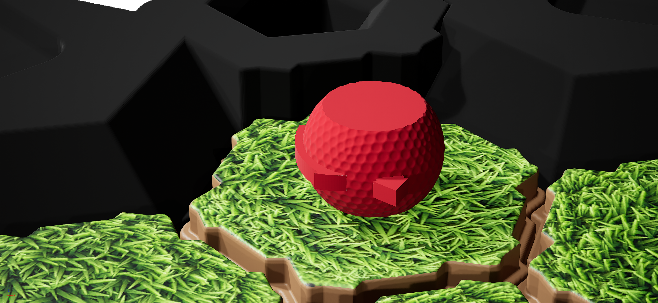
\includegraphics[width=1\linewidth]{chapters//generalInformation/Source Golf Ball.png}
\end{figure}

\subsection{Hexes}
Hexes are either land hexes or tile hexes. Hexes (and anything occupying them) that are next to each other are considered adjacent, regardless of any height difference. 

Water is the only type of tile hex included in this set. Tile hexes are considered to be one hex lower in elevation than land hexes. 
\end{document}